\chapter{Anforderungserhebung}

\section{Nutzer}
%Thesis Fragestellung aufgegriffen
    Um die Frage beantworten zu können, ob es möglich ist die übertragenen Daten der intelligenten Geräte, herstellerübergreifend überwachen zu können, ist es nötig Zugriff auf die eingehenden, sowie ausgehenden Daten der Geräte zu erhalten. In diesen Daten, welche vom \ac{IoT}-Gerät zum Broker und anders herum, geschickt werden befinden sich möglicherweise personenbezogene Daten sowie Hinweise auf mögliche Schwachstellen.
    Die nächste Herausforderung ist die gesammelten Daten auch einem Nutzer in einer aufbereiteten Ansicht zugänglich zu machen und die direkte Interaktion mit den Daten zu ermöglichen.

    Aus diesem Szenario heraus ergeben sich zwei wichtige Nutzerrollen.
    
%=====================================================================%    
%wer? Nutzerrolle: Admin (monitoring)
%=====================================================================%    
    Auf der einen Seite existiert der System- , Netwerkadministrator, welcher versucht Probleme in der Kommunikation zu finden und zu lösen oder eventuelle Anomalien zu erkennen.
%Aufgabenbereiche Motivation
    Nach Burgess \cite{burgess2004principles} zählen zu den Aufgabenbereichen von Netzwerk- und Systemadministratoren zählen unter anderem:
    \begin{itemize}
        \item \glqq Diagnostics, fault and change management\grqq{}
        
        Die Aufgabe der Administratoren in einem Unternehmen besteht unter anderem darin, Systeme für das eigene Unternehmen oder Kunden bereitzustellen und bei Problemen zu helfen. Um bei Problemen herausfinden zu können, wo das Problem entstanden ist und wie es schnell behoben werden kann, ist es hilfreich die Kommunikation im Netzwerk zu beobachten. Zum Beispiel kann erkannt werden, ob \ac{TCP}-Pakete überhaupt an dem Gerät ankommen oder schon auf dem Übertragungsweg verloren gehen. Abhängig davon, kann das Problem weiter eingeschränkt und irgendwann lokalisiert werden.
        
        \item \glqq Configuration and maintenance\grqq{}
        Für eine korrekte Konfiguration der Systeme ist es notwendig die Kommunikation nachvollziehen zu können. Dazu muss ein Verständnis der genutzten Technologien vorhanden sein. Des Weiteren sollte ebenfalls bekannt sein, welche Art von Daten mithilfe der Kommunikation übertragen werden.
        
        %Performance regarding bottlenect.
        Die Aufzeichnung von Datenpaketen, deren Größe und Zeitstempel ermöglichen mithilfe von statistischer Analyse, Rückschlüsse auf die Netzwerkbelastung.
        
        \item \glqq Application-level services\grqq{}
        
        %Reverse Proxies und DNS
        Auf dieser Ebene müssen Administratoren verschiedene Applikationen wie \ac{DNS}-Server\footnote{\glqq Das DNS verknüpft [...] Rechnernamen und IP-Adressen miteinander. Es leistet zusätzlich die Speicherung und Ausgabe weiterer Informationen über die Dienste, die mit einer Domain verknüpft sind \cite{denic_eg}.\grqq{}} oder Proxies konfigurieren und Anwendungen miteinander verbinden um neue Systeme in die bestehende Systemlandschaften zu integrieren.
        
        \item \glqq Network-level services\grqq{}
        
        Auch können verschiedene Protokolle miteinander verbunden werden.
        
    \end{itemize}

% Ziel
    Das Ziel eines Netzwerkadministrators ist somit die Identifikation von Störquellen sowie das sicherstellen der Verfügbarkeit aller geschäftskritischen Dienste (\emph{high availability}). Dies ist eine wichtige Voraussetzung für hohe Kundenzufriedenheit.
    
%was gibt es bereits (Wireshark) was kann die Software besser/kann nur die Software
    Wie bereits erwähnt, gibt es für die einzelnen Phasen verschiedene Tools die sich in der Praxis bereits etabliert haben und Anwender in ihrer Arbeit unterstützen.
    
    %https://proquestcombo.safaribooksonline.com/9781492020356
    Wireshark \cite{SandersChris2017Ppa}, ein Tool zum Überwachen und Aufzeichnen des Netzwerkverkehrs, beinhaltet die gleiche Funktionalität wie ein Teil der Proxy Komponente. Der unterschied besteht jedoch darin, das die Komponente zusätzlich direkt in die Kommunikation eingreifen können soll. Das bedeutet, dass Nachrichten verändert, fallengelassen oder erneut gesendet werden soll, was durch ein dediziertes Monitoring-Tool nicht möglich ist.
    
% Was müsste die eigene Software verbessern
    %Log Messages
    Der Nutzer möchte nun, wenn er mit diesem Programm arbeitet, den Proxy in den Modus \glqq intercept\grqq{} oder \glqq none intercept\grqq{} stellen können um Inhalte spezieller Clients einzeln und gezielt prüfen zu können ohne zu viele Daten anderer Geräte im Netzwerk zu erhalten.
    %View Messages
    Des Weiteren möchte der Nutzer die Nachrichten, welche durch den \glqq intercept\grqq{} Modus abgefangen wurden, aufgelistet und angezeigt werden.
    %View ClientInfos
    Für denn Fall, dass etwas nicht ordnungsgemäß funktioniert oder fehlerhaft Konfiguriert wurde, ist es ebenfalls relevant die Verbindungsdaten der einzelnen Proxy Clients mit einer Verknüpfung mit dem zu untersuchenden \ac{IoT}-Gerät einsehen zu können.
    
%=====================================================================%
%wer? Nutzerrolle: Security Auditor
%=====================================================================%
% Motivation
    Auf der anderen Seite existiert der Security Auditor oder auch Penetration Tester, welcher versucht Schwachstellen in der Kommunikation oder dem Gerät oder dem Endpunkt zu identifizieren.
% Ziel
    Dies ermöglicht auf der einen Seite den Hersteller, von dem der Tester beauftragt wird, die Produkte im Rahmen der Qualitätssicherung vor Veröffentlichung zu testen um Probleme zu vermeiden. Dies ist nicht für Vertrauen innerhalb der Branche wichtig, sondern auch in bestimmten Bereichen z.B. kritischen Infrastrukturen im Gesetz verankert.
    Auf der anderen Seite bestätigt es ebenfalls, dass der Dienst eines Unternehmens gute und effiziente Sicherheitsmechanismen korrekt implementiert hat um die Kundendaten vor Gefährdungen der Vertraulichkeit, Integrität oder Verfügbarkeit zu schützen.
    
    Eine weiterer wichtiger Untersuchungsgegenstand sind Personen- und Unternehmensbezogene Daten. Diese haben aufgrund von datenschutzrechtlichen Bestimmungen eine besonders hohe Priorität. Dies wird in Form von manueller oder regelbasierter Inspektion der Übertragung durchgeführt.
    
%Was für Arbeitsabläufe
    
    %wie: Wie hilft die Software dabei das Ziel zu erreichen
    Die in dieser Arbeit zu konzipierende Software soll den Tester mithilfe von passivem Scannen und abfangen der Kommunikation in Schritt 2 (\emph{Information Gathering}) und durch manipulieren sowie erneut senden der Nachrichten Schritt 5 (\emph{Exploitation}) unterstützen.
    
    %was gibt es bereits (Wireshark) was kann die Software besser/kann nur die Software
    Wie beim Netzwerkadministrator bereits geschildert, kann Wireshark zur Informationsbeschaffung verwendet werden.
    Da bei Wireshark viele verschiedene Protokolle unterstützt und auch sehr detaillierte Informationen angezeigt werden, passiert es schnell, dass durch die große Menge wichtige Bestandteile untergehen (\emph{visual clutter}) oder nur mit Aufwand gefunden werden.
    
    Burp Suite von PortSwigger bietet im Gegensatz zu Wireshark ebenfalls eine Proxy Komponente und kann somit, wie in diesem Tool geplant, die Nachrichten protokollieren bzw. überwachen sondern auch in die Kommunikation eingreifen. Der große Unterschied besteht darin, dass Burp Suite ausschließlich für HTTP/s und (Sec)Websocket Kommunikation zu verwenden ist und keinerlei Unterstützung für das \ac{MQTT}-Protokoll bietet. Man könnte die Idee jedoch am einfachsten mit dieser Lösung vergleichen, da auch eine ähnlich Bedienung von Vorteil wäre. Dadurch würden Nutzer eine geringere Einarbeitungszeit benötigen und auch die Akzeptanz steigern.

\section{Abgeleitete Anforderungen}
    Im Folgenden werden die werden Use-Cases aus den obigen Nutzerbeschreibungen extrahiert und beschrieben.
    %Aus Beschreibung ergeben sich Use-Cases
    \subsection{Use-Cases}
    \begin{figure}[h]%h=direkt danach t=top b=bottom
        \centering
        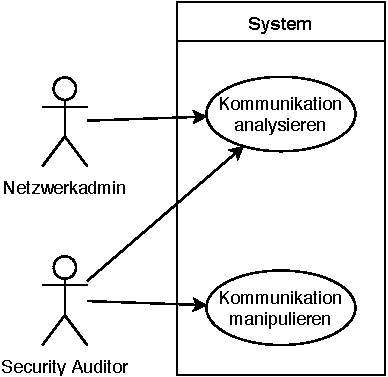
\includegraphics[width=7cm]{tex/bilder/3_anforderungen/Use-Case.pdf}
        \captionof{figure}{Use-Case Diagramm}
        \label{fig:use-case}
    \end{figure}
    
    Zum ersten Use-Case \emph{Kommunikation analysieren}:
    	Der Nutzer möchte die Nachrichten der \ac{MQTT}-Kommunikation analysieren.
    	Des Weiteren ist es notwendig das Abfangen der Nachrichten pro Gerät einstellen zu können, um nur die gewünschte Kommunikation und somit eine selektive Analyse zu ermöglichen.
    	Um dies zu bewerkstelligen, ist es notwendig die angezeigten Nachrichten nach den Inhalten zu filtern.
    	
    Zu \emph{Kommunikation manipulieren}:
        Im Folgenden werden Aktionen wie Payload ändern, Nachricht senden, Nachricht kopieren, Nachricht ändern bzw. speichern,Nachricht verwerfen beschrieben.
    	Der Nutzer möchte auf verschiedene Weisen die Kommunikation zwischen zwei Kommunikationspartnern über ein drittes System verändern können.
    	Durch Veränderung des Nachrichteninhalts einzelner Nachrichten ist es dem Nutzer möglich die Kommunikation zu verändern.
    	Anhand von selbsterstellten Pakete, welche im Namen der Kommunikationspartner erstellt werden, sollen vom Nutzer gewünschte Informationen übertragen werden.
    	Um die repetitive Arbeit der Nachrichtenerstellung zu reduzieren und die Arbeit zu beschleunigen, kann eine abgefangene Nachricht kopiert werden.
    	Diese Änderungen sollen anschließend gespeichert werden können um Nachrichten zu einem späteren Zeitpunkt versenden oder weiter Verändern zu können.
    	Für den Fall, dass übertragene Nachrichten Inhalte beinhalten, welche nicht ankommen dürfen oder nicht den gewünschten Inhalt haben, möchte der Nutzer sie verwerfen und somit von der Kommunikation entfernen.

    %Tabelle mit Funktionale Anforderungen
    \subsection{Formale Anforderungen}
    Anhand der Use-Cases lassen sich folgende formale Anforderungen ableiten (siehe Tabelle \ref{tab:functional_requirements}).
    Dabei ist zu beachten, dass diese Anforderungen, dadurch das es sich um ein abstraktes Konzept handelt, unspezifisch und ausschließlich funktional sind.
    \begin{table}[h]
        \centering
        \begin{tabular}{c|c}
            \hline
            $Nr.$ & $Name$ \\ \hline
            %Nachricht abfangen vllt auch ein Feature was nennenswert ist oder wird es m it Nr.3 abgedeckt???
            1 & Nachrichten anzeigen \\ \hline
            2 & Nachrichten filtern \\ \hline
            3 & Abfangen umschalten \\ \hline
            4 & Nachricht manipulieren \\ \hline
            5 & Nachricht senden \\ \hline
            6 & Nachricht verwerfen \\ \hline
        \end{tabular}
        \caption{Funktionale Anforderungen}
        \label{tab:functional_requirements}
    \end{table}
    
        \subsubsection{1. Nachrichten anzeigen}
        Das System ermöglicht die Anzeige von Nachrichten einer \ac{MQTT}-Kommunikation.
        Dabei werden diese in einer chronologischen Reihenfolge dargestellt und stellen relevante Informationen wie Topic, Payload, Quality of Service und Zeitpunkt der Übertragung zur Verfügung.
        
        \subsubsection{2. Nachrichten filtern}
        Die Software muss angezeigte Nachrichten nach deren Attributen filtern können.
        
        \subsubsection{3. Abfangen umschalten}
        Dem Nutzer muss die Möglichkeit gegeben werden, das Abfangen der  Kommunikation der \ac{IoT}-Geräte zu aktivieren oder deaktivieren.
        Dabei werden die Pakete nicht nur dupliziert, sondern dürfen auch nicht an den Kommunikationspartner weiter geleitet werden.
        Dies muss dem Nutzer pro verbundenem Gerät zur Verfügung konfigurierbar sein.
        
        \subsubsection{4. Nachricht manipulieren}
        Der Nutzer muss den Inhalt der aufgezeichneten Nachrichten verändern können.
        Vorrangig muss der übertragene Nachrichteninhalt als Text verändert werden können.
        
        \subsubsection{5. Nachricht senden}
        Es muss garantiert werden, dass eigene Nachrichten gesendet werden können.
        Das Senden beinhaltet nicht nur das senden neuer Nachrichten, sondern umfasst auch das erneute senden (\emph{replay attack}) von bereits übertragenen Nachrichten. Die Inhalte werden in diesem Fall nicht verändert und wie erfasst erneut versendet.
        
        \subsubsection{6. Nachricht verwerfen}
        Das System muss es dem Nutzer ermöglichen, abgefangene Nachrichten verwerfen zu können.
        Dies bedeutet, dass gesendete Inhalte nicht an den gewünschten Kommunikationspartner weitergeleitete werden, sondern nachdem sie abgefangen wurden aus der Kommunikation entfernt werden.
        Die ausgewählten Nachrichten werden somit auch in der Oberfläche nicht weiter angezeigt.
        
        